%--------------------------------------------
% Chapter: REMOTE CONTROL UNIT: GRAUPNER PPM DECODING
%--------------------------------------------
\chapter{Remote Control Unit: PPM Decoding}
\label{sec:remoteControl}

%- - - - - - - - - - - - - - - - - - - - - - 
% Section: Graupner PPM Signal in a nutshell
%- - - - - - - - - - - - - - - - - - - - - - 
\section{Graupner PPM sum signal in a nutshell}
\label{sec:remoteControl:ppmNutshell}

The HElikopter Team of Hochschule Esslingen uses the Graupner radio remote control system to control the Quadrocopters. Therefore, it is necessary to decode the Graupner PPM Signal delivered by the radio receiver to give a user's input to the controller platform of the Quadrocopters.

The Graupner remote control is a multi-channel system that comprises the transmission of up to 12 channels. Each individual channel is encoded by a PWM signal with a periode time of 20ms (resulting in a update rate of 50Hz) as depicted in fig. \ref{fig:remoteControl:ppmNutshell:pwmSignal}. According to the transmitted value of each channel, the on-time $T_{on}$ varies between 1ms (min. value) and 2ms (max. value).

\begin{figure}[H]
    \centering
    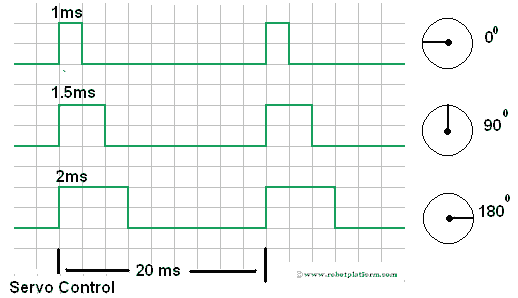
\includegraphics[width=0.7\textwidth]{fig/ch-ppm-kernel-driver/graupnerPWM}
    \caption[PWM signal scheme of a RC servo \cite{doc:RPL}]{PWM signal to control a RC servo \cite{doc:RPL}}
    \label{fig:remoteControl:ppmNutshell:pwmSignal}
\end{figure}


In order to transmit several (up to 12) PWM channels simultaneously, all channels are combined sequentially in one sum signal as depicted in fig. \ref{fig:remoteControl:ppmNutshell:ppmSumSignal}. This results in a PPM signal with a fixed pulse width. The time between the rising edges of two individual pulses encodes the on-time of the PWM signal of the corresponding channel. The remaining pause gap at the end of a PPM frame is used to resynchronize the transmission. Without this resynchronization, it would be impossible to map from a received pulse to the corresponding channel number. 

\begin{figure}[H]
    \centering
    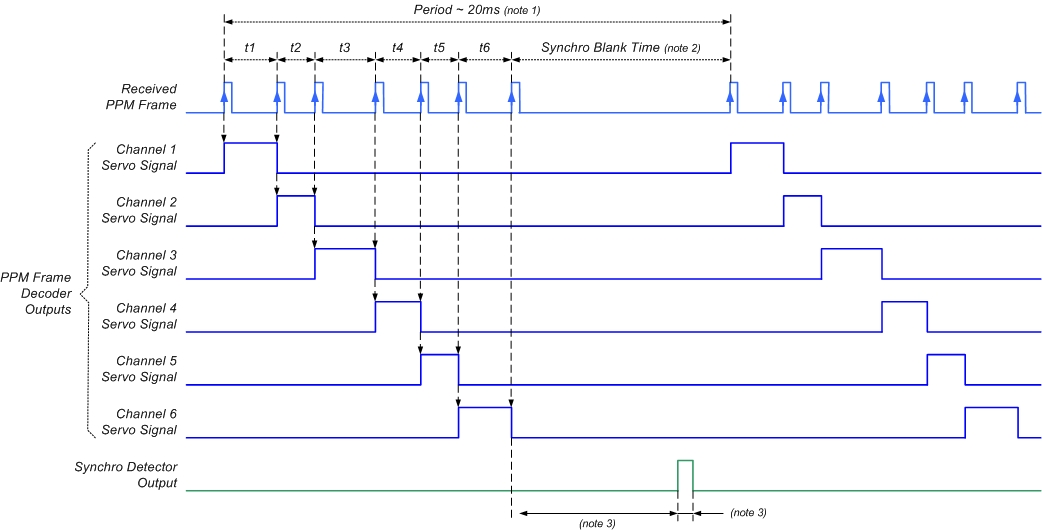
\includegraphics[width=\textwidth]{fig/ch-ppm-kernel-driver/graupnerPPM}
    \caption[PPM sum signal scheme \cite{doc:REP}]{PPM sum signal scheme of an exemplary 6 channel remote control \cite{doc:REP}}
    \label{fig:remoteControl:ppmNutshell:ppmSumSignal}
\end{figure}

Some Graupner systems have the same sum signal encoding, but with a inverted out signal (high-state becomes low-state, and vice-versa). But if triggered on rising or falling edges only, this fact will not harm the general encoding/decoding approach.

%- - - - - - - - - - - - - - - - - - - - - - 
% Section: Building a custom kernel driver
%- - - - - - - - - - - - - - - - - - - - - - 
\section{Building a custom kernel driver}
\label{sec:remoteControl:kernModule}

To build a custom kernel driver it is mandatory to have all Linux kernel sources on your development machine. If this is not already the case, please see chapter \ref{sec:OS} on how to get the latest kernel sources and how to build a custom kernel.

Furthermore, it is crucial that the kernel sources have the same version number as the kernel installed on the Raspberry Pi's firmware! Due to that fact, it is recommended to perform a kernel update and subsequently compile the custom kernel driver.

Below in listing \ref{code:remoteControl:kernModule:makefile}, a generic \texttt{Makefile} is shown to cross-compile a custom kernel driver for the Raspberry Pi. The variable \texttt{KDIR} in line 7 specifies the path to the kernel sources. The variable \texttt{CROSS\_COMPILE} in line 6 specifies the path to the raspberry pi cross-compile tools. Depending on the distribution and development environment, these paths may have to be adapted.

In line 11 of listing \ref{code:remoteControl:kernModule:makefile} the object file (with file extension \texttt{.o}) of the compilation process that shall be linked as a kernel module file (file extension \texttt{.ko}) gets defined. If another kernel driver file shall be compiled, put the c-code file name there and change the file extension to \texttt{.o}.

\begin{lstlisting}[language=bash,caption={[Simple Makefile to compile a custom kernel driver]Simple Makefile to compile a custom kernel driver (here for the kernel module \texttt{ppmDemux})},label=code:remoteControl:kernModule:makefile,otherkeywords={ifeq,else,ifneq,endif,default,clean}]
ARCH := arm
UNAME := $(shell uname -m)
ifeq ($(UNAME),armv6l)
	KDIR := /usr/src/linux/
else
	CROSS_COMPILE:=/home/user/rpi/tools/arm-bcm2708/gcc-linaro-arm-linux-gnueabihf-raspbian-x64/bin/arm-linux-gnueabihf-
	KDIR := /home/user/rpi/linux/
endif

ifneq ($(KERNELRELEASE),)
	obj-m := ppmDemux.o
else

default:
	$(MAKE) ARCH=$(ARCH) CROSS_COMPILE=$(CROSS_COMPILE) -C $(KDIR) M=$(PWD) modules
endif

clean:
	rm -rf *.ko *.o .*.cmd .tmp_versions Module.symvers
	rm -rf modules.order *.mod.c
\end{lstlisting}
In the case of the \texttt{ppmDemux} kernel driver, a free running 64bit counter (called \texttt{System Timer}\footnote{See the peripherals datasheet on Raspberry Pi's SoC \href{https://www.raspberrypi.org/documentation/hardware/raspberrypi/bcm2835/BCM2835-ARM-Peripherals.pdf}{Broadcom BCM2835}, p. 172 ll. }) of the Raspberry Pi's System on Chip (SoC) has been used to determine a precise timing. This free running counter runs on $1Mhz$ independently of all other peripherals. This results in a maximum accuracy of $1\mu s$ of all measurements that utilize the \texttt{System Timer}.

The hardware address of the \texttt{System Timer} is defined by the base address \texttt{0x7E003000} plus the offset of the required data register (see \cite{doc:bcm2835}, p. 175 ll.). Due to the \texttt{MMU} of the BCM2835 chip, the physical hardware address gets translated to the I/O base address \texttt{0x20003000} (as defined in line 27 of listing \ref{code:append-ppmDemuxCode:ppmDemux}). This address has to be used in the kernel module driver to access the free running $1Mhz$ \texttt{System Timer}.

Based on the articles \cite{doc:Kern70} and \cite{doc:Kern81}, a kernel driver has been developed, to process a hardware trigger on GPIO pin 24. Whenever a rising edge is detected, a hardware interrupt is issued to the Kernel. The interrupt behavior in rising edges is defined in line 96 of listing \ref{code:append-ppmDemuxCode:ppmDemux}. The Interrupt Service Routine (ISR) is called in consequence (defined as function \texttt{hard\_isr} in line 60 ll. of listing \ref{code:append-ppmDemuxCode:ppmDemux}). 
\begin{lstlisting}[firstnumber=60]
static irqreturn_t hard_isr( int irq, void *dev_id )
{
	/* read free running timer (64bit) @ 1MHz */
	modIrqObj.timer_l = readl(timer_low);
	modIrqObj.timer_h = readl(timer_high);

	/* counts rising edges since last read */
	modIrqObj.irqNum += 1;

	return IRQ_WAKE_THREAD;
}
\end{lstlisting}
This Interrupt Service Routine is the first function called whenever a rising edge event on GPIO24 occurs. The value of the 64bit \texttt{System Timer} get read out and an interrupt counter gets increased. That way, even for the unprobable case that one interrupt gets unprocessed, the synchronization of the Graupner PPM sum signal can be guaranteed.

After the hard ISR\footnote{Code inside of the hard ISR should be reduced to the absolute minimum and only necessary tasks should be performed. Every unnecessary CPU cycle in this section will slow down the system performance dramatically!} has been processed, the threaded interrupt handler \texttt{rpi\_gpio\_isr} (line 52 ll. of listing \ref{code:append-ppmDemuxCode:ppmDemux}) gets called. For complex kernel drivers, in this function can be implemented complex algorithms to process the captured signals. This function is threaded and can be prioritized by the kernel's scheduler to guarantee a minimal latency time of the system.
\begin{lstlisting}[firstnumber=60]
static irqreturn_t hard_isr( int irq, void *dev_id )
{
	/* read free running timer (64bit) @ 1MHz */
	modIrqObj.timer_l = readl(timer_low);
	modIrqObj.timer_h = readl(timer_high);

	/* counts rising edges since last read */
	modIrqObj.irqNum += 1;

	return IRQ_WAKE_THREAD;
}
\end{lstlisting}
When all statements of the soft (threaded) ISR \texttt{rpi\_gpio\_isr} has been processed, the read function of the kernel driver get waken up (see listing \ref{code:append-ppmDemuxCode:ppmDemux} in line 55 and line 118 for the counterpart in the read function).
\begin{lstlisting}[firstnumber=52]
static irqreturn_t rpi_gpio_isr( int irq, void *data )
{
	/* wake up read function to retrieve new data */
	wake_up( &sleeping_for_ir );
\end{lstlisting}
\vspace{-0.7cm}
\begin{lstlisting}[firstnumber=117]
	/* wait for an rising edge event (caught by ISR) */
	wait_event_interruptible( sleeping_for_ir, modIrqObj.irqNum);
\end{lstlisting}

The complete code of the \texttt{ppmDemux} kernel module driver can be seen in listing \ref{code:append-ppmDemuxCode:ppmDemux} and in the SVN repository in \texttt{/impl/trunk/kern/}.

In order to compile the kernel driver, navigate to folder where the c code files and the \texttt{Makefile} are located and execute the following command in the bash command line:
\begin{lstlisting}[language=bash,otherkeywords={make}]
cd ../path/to/kernelDriverFiles/
make
\end{lstlisting}

This will produce the compile kernel module object file \texttt{ppmDemux.ko}. If the kernel module has been cross-compiled on the Development Environment (VM) then copy this \texttt{.ko}-file to the Raspberry Pi's file system by using scp.
\begin{lstlisting}[language=bash,otherkeywords={scp}]
scp ./ppmDemux.ko pi@192.168.2.1:~/
\end{lstlisting}

In the above shown command, the kernel module object file will be copied to the home directory of the user \texttt{pi} on the Raspberry Pi's Linux system. If the IPv4 address has been changed, this has to be adapted when using the above stated command (here used: standard IP address of pre-configured Raspberry Pi Firmware).

After the file transfer is finished, the kernel module can be loaded to the Linux System. Navigate to the location of the stored kernel module object file (in this example the home directory of the user \texttt{pi}) and use the command \texttt{insmod}.
\begin{lstlisting}[language=bash,otherkeywords={insmod, sudo}]
cd /home/pi/
sudo insmod ppmDemux.ko
\end{lstlisting}

If the kernel module is successfully loaded (no error messages occurred), then a character file handler \texttt{/dev/gpioirq24} has been created by the kernel module driver \texttt{ppmDemux}. Get noticed of rising edges on GPIO pin 24, read the character file handler \texttt{/dev/gpioirq24} as shown in the exemplary test code as shown in listing \ref{code:append-ppmDemuxCode:ppmDemusReader} or file \texttt{getPpmDemuxValues.c} in the SVN repository folder \texttt{/impl/trunk/kern/tst/}.

%- - - - - - - - - - - - - - - - - - - - - - 
% Section: Stimulating the GPIO-Pins
%- - - - - - - - - - - - - - - - - - - - - - 
\section{Stimulating the GPIO-Pins for validation}
\label{sec:remoteControl:stimuli}

For testing and validation purposes of the custom built Kernel Driver \texttt{ppmDemux} of chapter \ref{sec:remoteControl:kernModule}, it was required to stimulate the GPIO pin 24 with a PPM signal similar to a Graupner sum signal.

For this purpose, a STM32F4 Discovery board was used to run a specifically written firmware that produces a variable PPM signal as depicted in fig. \ref{fig:remoteControl:stimuli:hwSetup}. The firmware of the STM32F4 board is capable to produce PPM signals with a pulse-to-pulse with of $480\mu s$ up to $2560\mu s$. By pressing the \texttt{blue button} of the STM32F4 Discovery board as shown in fig. \ref{fig:remoteControl:stimuli:hwSetup}, the pulse-to-pulse width can be altered in the sequence as shown on table \ref{tab:remoteControl:stimuli:stm32f4States}.

\begin{figure}[H]
    \centering
    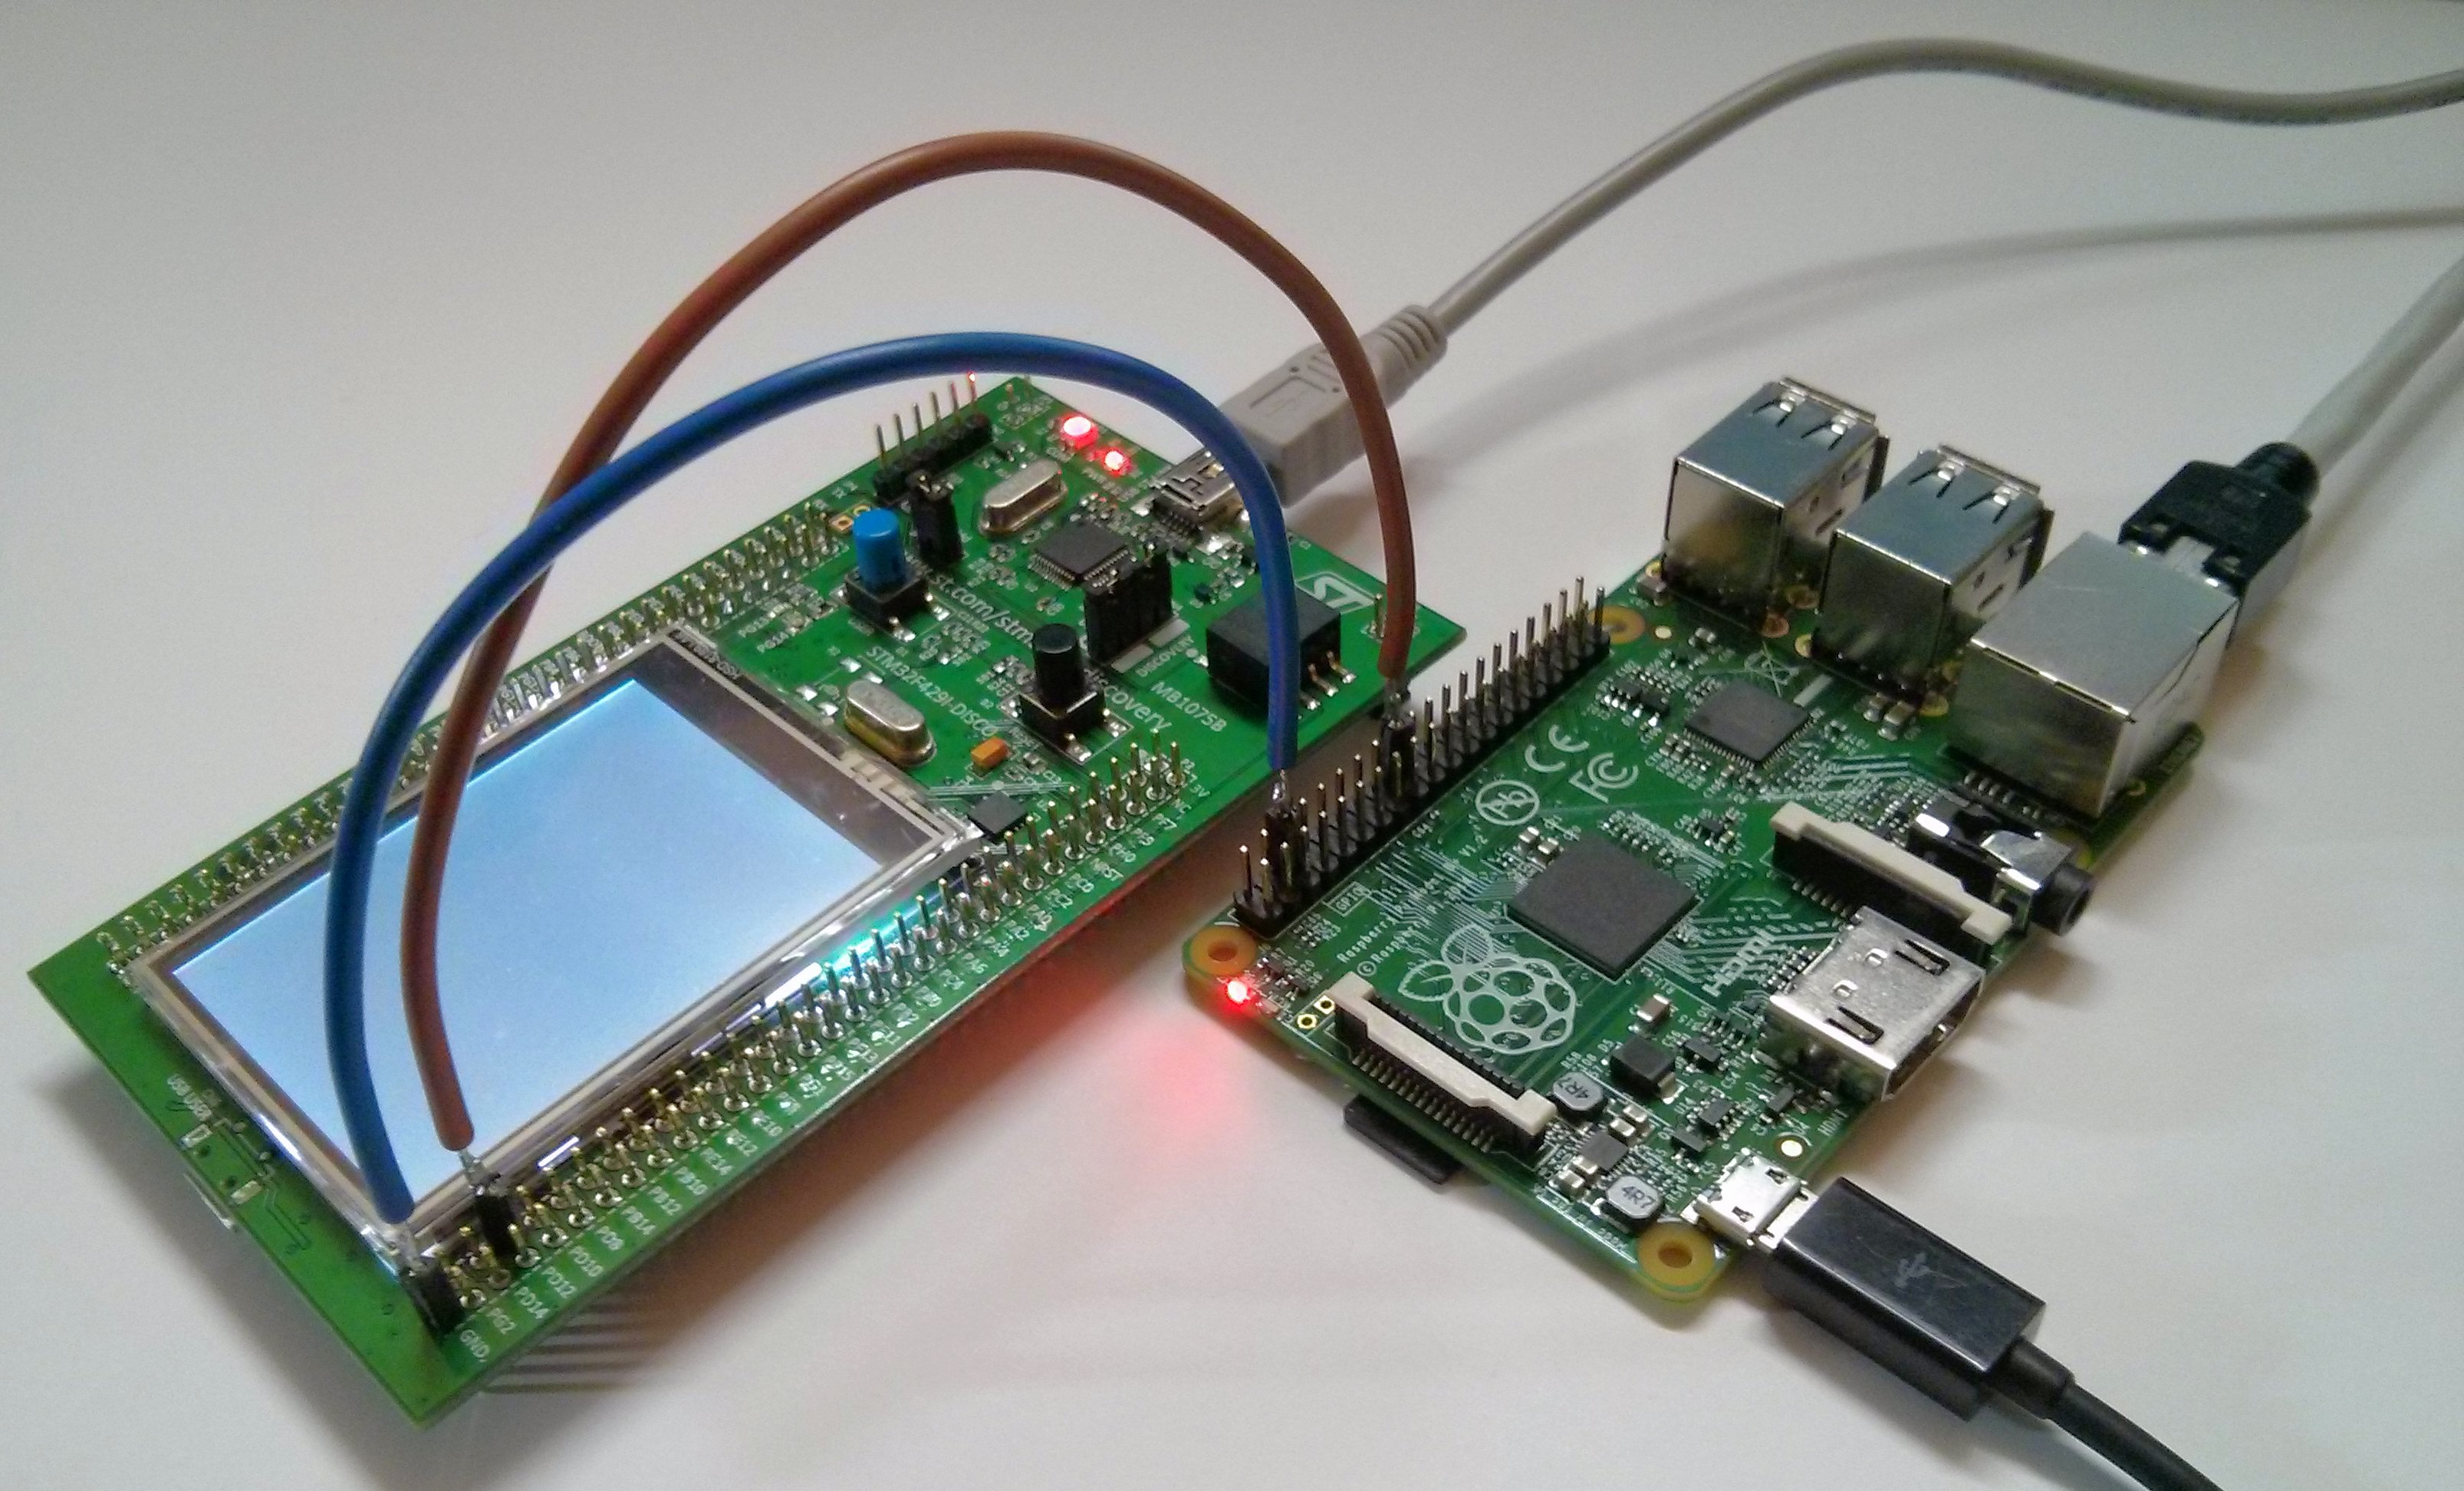
\includegraphics[width=0.80\textwidth]{fig/ch-ppm-kernel-driver/picStimulusRpi}
    \caption[Stimulating GPIO Pins of Raspberry Pi]{In order to test the PPM kernel driver, a STM32F4 Discovery Board was used to stimulate the GPIO Pin 24 of Raspberry Pi Board. The signals got also observed by a 50 MHz Oscilloscope to validate the measured PPM length.}
    \label{fig:remoteControl:stimuli:hwSetup}
\end{figure}

The firmware developed for the STM32F4 Discovery board can be found in the SVN repository in \texttt{/impl/trunk/kern/tst/STM32F4\_PWM\_Stimulator}. To use the firmware, first the CooCox IDE\footnote{http://www.coocox.org/software/coide.php} has to be installed on the development machine as well as the GCC Toolchain for ARM Embedded Processors\footnote{https://launchpad.net/gcc-arm-embedded/+download}. Then the provided project file in the SVN repository can be opened and customized, if needed.

\begin{table}[H]
\centering
	\begin{tabular}{c|c||c|c}
\hline
\textbf{State No.} & \textbf{Pulse-to-pulse witdth} & \textbf{State No.} & \textbf{Pulse-to-pulse witdth}\\
\hhline{=|=#=|=}
1 & $480\mu s$ & 10 & $1590\mu s$\\
2 & $620\mu s$ & 11 & $1710\mu s$\\
3 & $730\mu s$ & 12 & $1840\mu s$\\
4 & $860\mu s$ & 13 & $1960\mu s$\\
5 & $970\mu s$ & 14 & $2080\mu s$\\
6 & $1100\mu s$ & 15 & $2200\mu s$\\
7 & $1220\mu s$ & 16 & $2320\mu s$\\
8 & $1350\mu s$ & 17 & $2440\mu s$\\
9 & $1460\mu s$ & 18 & $2560\mu s$\\
\hline
	\end{tabular}
	\caption[Pulse-to-pulse width of STM32F4 firmware states]{Pulse-to-pulse width in microseconds for each state of the STM32F4 firmware}
	\label{tab:remoteControl:stimuli:stm32f4States}
\end{table}

\begin{figure}[H]
    \centering
    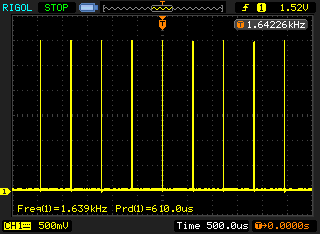
\includegraphics[width=0.60\textwidth]{fig/ch-ppm-kernel-driver/osci_ppm_610us}
    \caption[Oscilloscope graph of stimulus signal (610µs)]{Oscilloscope graph of stimulus signal emitted by the STM32F4 Discovery board (Custom STM32F4 firmware for 610$\mu$s pulse-to-pulse width).}
    \label{fig:remoteControl:stimuli:oszi610}
\end{figure}

To validate the stimulus signal output of the STM32F4 Discovery board, the output signals where observed with a 50Mhz oscilloscope. Screenshots of two PPM signals are shown in fig. \ref{fig:remoteControl:stimuli:oszi610} and fig. \ref{fig:remoteControl:stimuli:oszi1220}.

\begin{figure}[H]
    \centering
    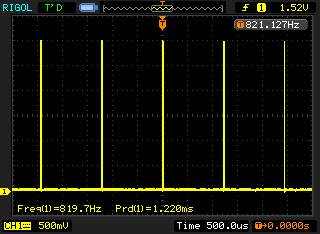
\includegraphics[width=0.60\textwidth]{fig/ch-ppm-kernel-driver/osci_ppm_1220us}
    \caption[Oscilloscope graph of stimulus signal (1220$\mu$s)]{Oscilloscope graph of stimulus signal emitted by the STM32F4 Discovery board (Custom STM32F4 firmware for 1220$\mu$s pulse-to-pulse width).}
    \label{fig:remoteControl:stimuli:oszi1220}
\end{figure}

%- - - - - - - - - - - - - - - - - - - - - - 
% Section: Results on experimental kernel driver
%- - - - - - - - - - - - - - - - - - - - - - 
\section{Results on experimental kernel driver}
\label{sec:remoteControl:results}

Before the custom kernel module driver \texttt{ppmDemux} has been developed by the authors of this document, a performance test of the standard Kernel's GPIO interface has been evaluated. For this purpose, a $1220\mu s$ PPM signal was generated (as shown in chapter \ref{sec:remoteControl:stimuli}) and measured with a simple test script.

The measured pulse-to-pulse time was measured under system idle and system under full load. The 'system under full load' scenario was produced by executing 3 threads that run at full load as well as 3 threads that produce full I/O-load. To achieve this, the program \texttt{stress} was installed on the Raspberry Pi's Linux system by issuing the command shown below on the Raspberry Pi's bash command line
\begin{lstlisting}[language=bash,otherkeywords={sudo,tar,touch,gedit,cp,apt-get,mkdir}]
sudo apt-get install stress
\end{lstlisting}

To set the test system under a full load scenario, the command \texttt{stress} got issued as shown below:
\begin{lstlisting}[language=bash,otherkeywords={sudo,tar,touch,gedit,cp,apt-get,mkdir}]
sudo stress -c 3 -i 3 &
\end{lstlisting}
This command starts 3 threads that each consume the max. CPU cycles available\footnote{The ampersand character (\texttt{\&}) at the end of the line runs the processes in the background of the system. To stop the program \texttt{stress} type the command '\texttt{sudo killall stress}' to the bash command line. This will terminate all processes of the program \texttt{stress} and set the system back to an idle state.}. Additonally 3 threads are started that each put a max. I/O load on the system. This setup can be considered as a maximum load scenario for a the single core Raspberry Pi B+ board.

For each scenario (idle and full load), approximately 10000 measurements where taken and stored. In fig. \ref{fig:remoteControl:results:stdKernIdle} and fig. \ref{fig:remoteControl:results:stdKernLoad} the results of these measurements can be seen.

When using the standard Kernel's GPIO interface, the accuracy of the measurement under system idle is still in a acceptable range although latency jitter exceeds the acceptable range in rare cases (compare with fig. \ref{fig:remoteControl:results:stdKernIdle}).

\begin{figure}[H]
    \centering
    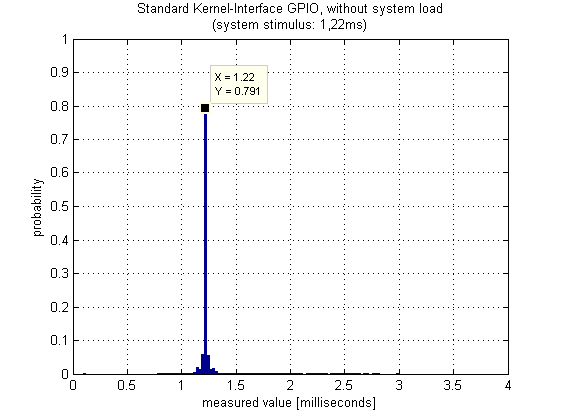
\includegraphics[width=0.75\textwidth]{fig/ch-ppm-kernel-driver/stdKern_woLoad}
    \caption[Measured pulse period time with standard kernel (system on idle)]{Measured pulse period time with standard kernel's GPIO interface \\(system on idle)}
    \label{fig:remoteControl:results:stdKernIdle}
\end{figure}

On the other hand, when the system is under full load the latency jitter exceeds the acceptable range by far. As in fig. \ref{fig:remoteControl:results:stdKernLoad} can be seen, approximately 25\% of all measured pulse-to-pulse widths are missed. This results in measured pulse-to-pulse width that is double the width of the stimulus signal. The second spike at $2.5ms$ indicates this effect. Unfortunately, for a mechanism to measure the user's remote control input, this is a unacceptable situation.

Therefore, the development of a custom kernel module driver called \texttt{ppmDemux} has been started. The proof-of-concept approach of chapter \ref{sec:remoteControl:kernModule} has been tested under a Preempt\_RT patched Kernel environment, as shown in chapter \ref{sec:OS:preemptRtPatch}.

\begin{figure}[H]
    \centering
    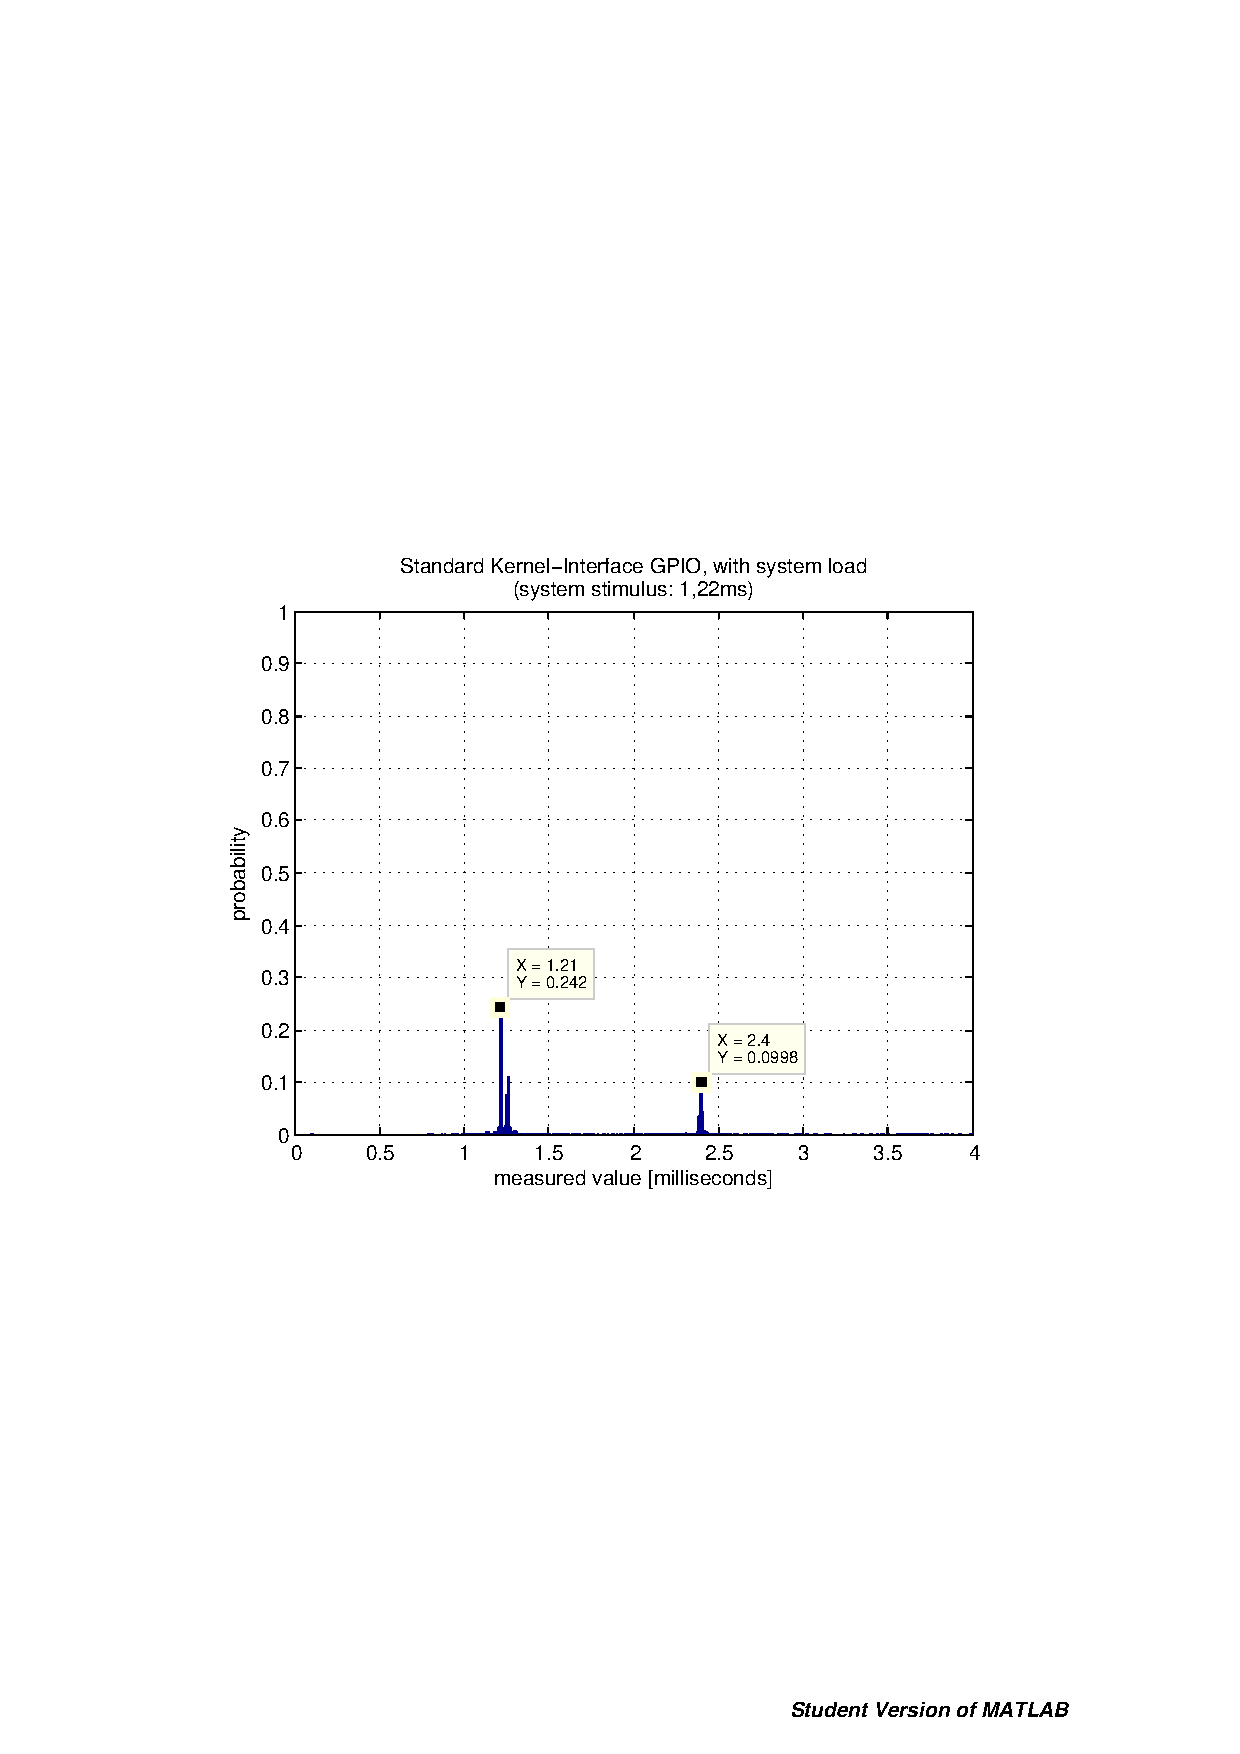
\includegraphics[width=0.75\textwidth]{fig/ch-ppm-kernel-driver/stdKern_withLoad}
    \caption[Measured pulse period time with standard kernel (system under full load)]{Measured pulse period time with standard kernel's GPIO interface (system under full load). The second spike at 2.4ms shows that many rising edges of the stimulus signal are missed. This is a non-acceptable result for a reliable system.}
    \label{fig:remoteControl:results:stdKernLoad}
\end{figure}

The custom kernel driver \texttt{ppmDemux} has been test again under the two test scenarios: system idle and system under full load (using the command \texttt{stress}). Under system idle conditions, fortunately the measured results are very good. The latency is negligible small and the latency jitter has a variance of roughly $10\mu s$ for a stimulus PPM signal with a pulse-to-pulse width of $1220\mu s$ (as shown in fig. \ref{fig:remoteControl:results:customKernIdle}). With some post-processing filters, a measurement accuracy of 1\%-3\% is a very realistic range for a future implementation.

Fortunately, even under heavy system load (full load scenario), the latency is again negligible. Also the latency jitter rises only marginally. A variance of not more than $53\mu s$ for a stimulus PPM signal under full load can be assumed (as depicted in fig. \ref{fig:remoteControl:results:customKernLoad}). No single edge of the PPM signal has been missed. Since the measurement shows a robust and reliable measurement behavior of the custom kernel driver, this approach is considered to be acceptable for the high reliability requirements of this project.

\begin{figure}[H]
    \centering
    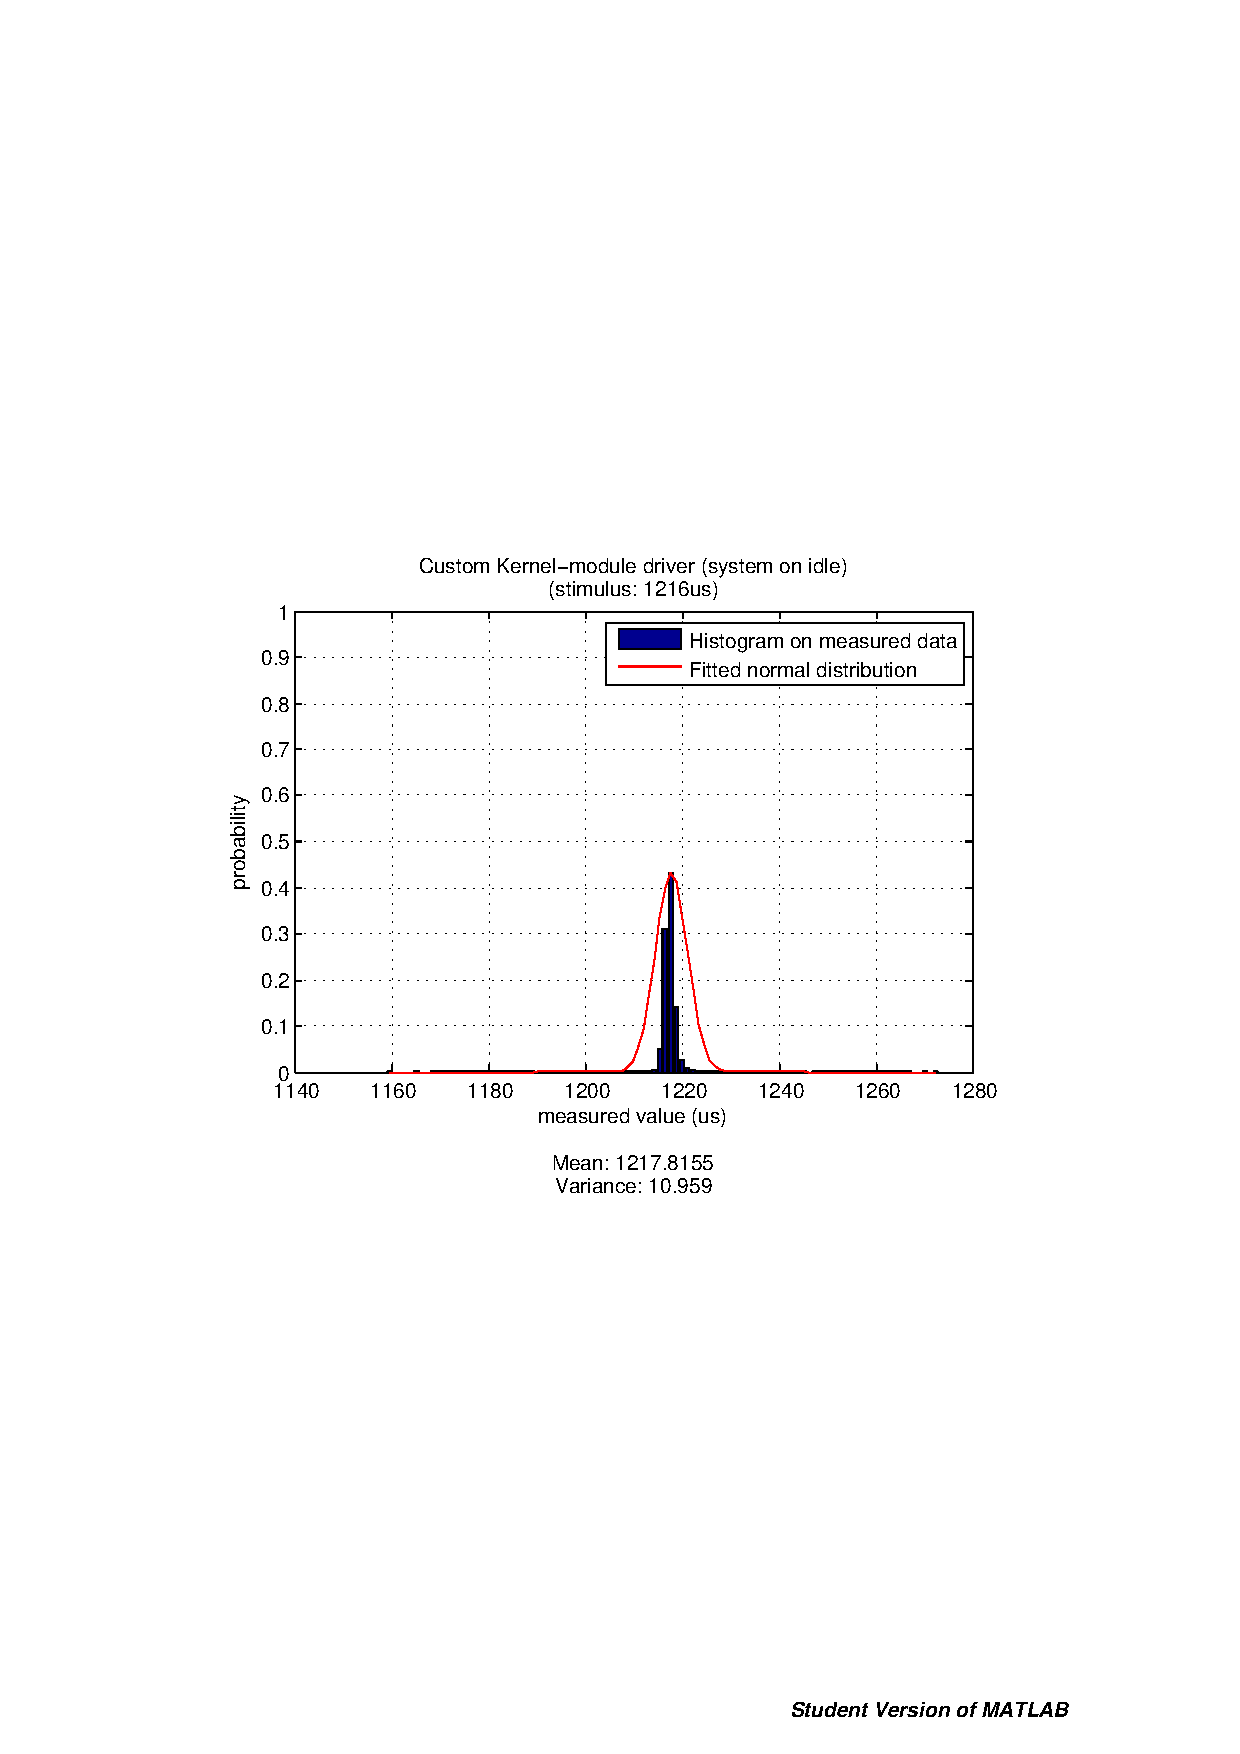
\includegraphics[width=0.71\textwidth]{fig/ch-ppm-kernel-driver/customKern_woLoad}
    \caption[Measured pulse period time with \texttt{ppmDemux} (system on idle)]{Measured pulse period time with \texttt{ppmDemux} (system on idle). The very low latency jitter shows the superior performance of the kernel driver approach.}
    \label{fig:remoteControl:results:customKernIdle}
\end{figure}

\begin{figure}[H]
    \centering
    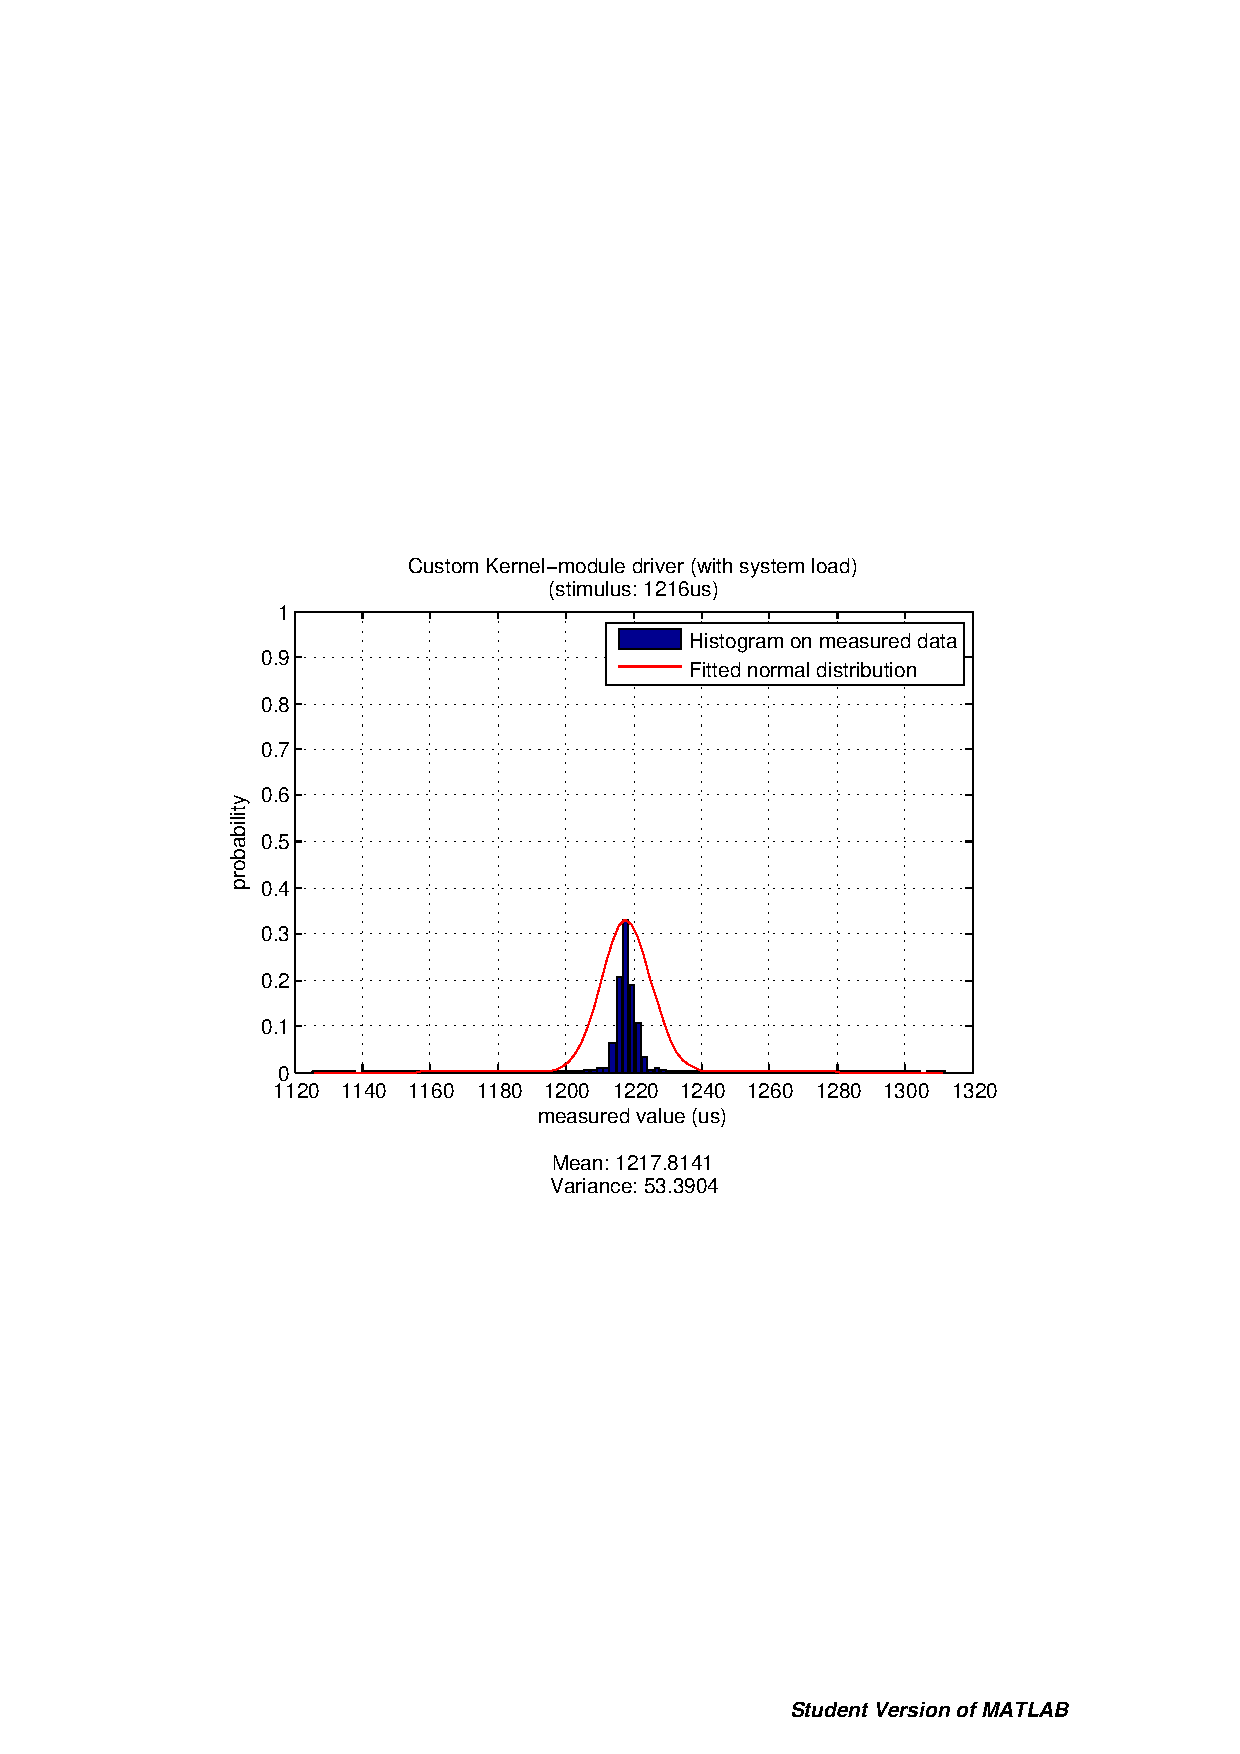
\includegraphics[width=0.71\textwidth]{fig/ch-ppm-kernel-driver/customKern_withLoad}
    \caption[Measured pulse period time with \texttt{ppmDemux} (system under full load)]{Measured pulse period time with \texttt{ppmDemux} (system under full load). Even under system's full load, the latency jitter is in an acceptable range. No single rising edge of the stimulus signal is missed. This shows that the kernel driver approach is the best choice for the high reliability requirements of this project.}
    \label{fig:remoteControl:results:customKernLoad}
\end{figure}